% !TeX root = ../../Book1.tex
% 纲要标题：### 7.3 平面闭曲线的绕转
% 纲要位置：几何学计划纲要.md，第 383 行。
% 正文状态：初稿；尚未正式审核。

% 纲要内容开始
% 
% * 切向映射的次数
% * 转角定理与简单闭曲线
% * 曲率符号、凸性及反例
% 
% 纲要内容结束

\section{平面闭曲线的绕转}
\label{g1:sec:0703}

沿一条平面闭曲线走一周，位置回到原点，切向量也回到原方向；但连续记录的切向角可能多转了几周。这个整周差把局部的有向曲率同闭曲线的整体形状联系起来。简单性将这个整数限制为 \(1\) 或 \(-1\)，曲率同号则使切向角单调，从而把转角与凸性联系起来。

\subsection{切向映射的次数}
\label{g1:subsec:0703:01}

设 \(\gamma:\mathbb R/L\mathbb Z\rightarrow\mathbb R^2\) 是 \(C^1\) 正则闭曲线；用弧长参数时，\(L\) 是总长，\(T(s)=\gamma'(s)\in S^1\)。闭合在这里包含参数接点的导数相容，因而 \(T(0)=T(L)\)。\cref{g1:lem:circle-angle-lift}说明，给定初始角度后，可以沿区间 \([0,L]\) 唯一地选择连续函数 \(\theta\)，使
\[
	T(s)=(\cos\theta(s),\sin\theta(s)).
\]
前章把圆周角度按整周归一为 \(e^{2\pi iu}\)；本节使用弧度，所以这里的 \(\theta\) 是那里角度提升的 \(2\pi\) 倍。等式 \(T(0)=T(L)\) 只保证 \(\theta(L)-\theta(0)\in2\pi\mathbb Z\)，不要求这个差为零。

\begin{definition}[旋转次数]\label{g1:def:rotation-index}
	设 \(P>0\)，\(\gamma:\mathbb R/P\mathbb Z\to\mathbb R^2\) 为 \(C^1\) 正则闭曲线，令 \(T(t)=\gamma'(t)/\|\gamma'(t)\|\)，并取 \(T\) 在 \([0,P]\) 上的连续角度提升 \(\theta\)。单位切向映射的\term[cishu]{次数}[degree]称为曲线的\term[xuanzhuancishu]{旋转次数}[rotation index]，记为
	\[
		\operatorname{rot}(\gamma)\coloneqq\deg T
		=\frac{\theta(P)-\theta(0)}{2\pi}\in\mathbb Z.
	\]
	若采用弧长参数，则以总长 \(L\) 替代 \(P\)。这里次数就是\cref{g1:thm:circle-fundamental}中圆周映射沿定义域正向一周的绕数；任意两个角度提升相差常数 \(2\pi m\)，故右边不依赖初始角度的选择。
\end{definition}

切向映射在方向圆周上走，原曲线在位置平面上走。旋转次数记录前者，不能与原曲线绕某个指定点的绕数混同：后者需要先选一个不在曲线上的点，而前者不需要这样一个点。

\begin{proposition}[有向曲率的整周积分]\label{g1:prop:total-turning}
	设 \(\gamma:\mathbb R/L\mathbb Z\rightarrow\mathbb R^2\) 是 \(C^2\) 弧长参数正则闭曲线，\(k\) 是按 \(T'=kJT\) 定义的有向曲率，其中 \(J(x,y)=(-y,x)\)。则其连续切向角提升是 \(C^1\) 的，且
	\begin{equation}\label{g1:eq:total-signed-curvature}
		k(s)=\theta'(s),\qquad \int_0^L k(s)\,\mathrm{d}s=2\pi\operatorname{rot}(\gamma).
	\end{equation}
	对一般正则参数 \(t\in[0,P]\)，同一公式写为
	\[
		2\pi\operatorname{rot}(\gamma)
		=\int_0^P\frac{\det(\dot\gamma(t),\ddot\gamma(t))}{|\dot\gamma(t)|^2}\,\mathrm{d}t.
	\]
\end{proposition}
\begin{proof}
	在任一小开弧上，圆周有光滑角度坐标。连续提升在这样的坐标区间内与该局部角度相差固定的 \(2\pi\) 整数倍，所以它具有与 \(T\) 相同的 \(C^1\) 正则性。微分给出
	\[
		T'(s)=\theta'(s)(-\sin\theta(s),\cos\theta(s))=\theta'(s)JT(s).
	\]
	与有向曲率的定义比较得到 \(k=\theta'\)，然后应用微积分基本定理。一般参数下，\cref{g1:prop:arc-length-param}给出 \(\mathrm{d}s=|\dot\gamma|\,\mathrm{d}t\)，而有向曲率公式为 \(k=\det(\dot\gamma,\ddot\gamma)/|\dot\gamma|^3\)；将这两个等式相乘即得最后一式。
\end{proof}

\begin{proposition}[方向与连续变形]\label{g1:prop:rotation-invariance}
	旋转次数在保向正则重参数化和保向平面刚体运动下不变；反向重参数化或平面反射各使它变号。若 \(\gamma_u:\mathbb R/P\mathbb Z\rightarrow\mathbb R^2\) 是一族闭曲线，\((t,u)\mapsto\gamma_u(t)\) 与 \((t,u)\mapsto\partial_t\gamma_u(t)\) 均连续，且后者处处非零，\(u\in[0,1]\)，则 \(\operatorname{rot}(\gamma_u)\) 与 \(u\) 无关。
\end{proposition}
\begin{proof}
	保向重参数化只按原次序走过切向映射；反向重参数化使切向量成为原切向量的负向并逆序走过。取负向只给切向角加上 \(\pi\)，逆序则把总增量变号。保向平面刚体运动给角度加一个常数，反射把角度变为某个常数减去原角度，这证明前两句。

	对连续变形，单位切向量
	\[
		T_u(t)=\frac{\partial_t\gamma_u(t)}{|\partial_t\gamma_u(t)|}
	\]
	构成圆周映射的连续同伦。把平面识别为复平面，考虑 \(T_u(t)/T_u(0)\)，就得到基点始终为 \(1\) 的环路同伦。\cref{g1:thm:circle-fundamental}的同伦不变性使它们的绕数相同，而除以 \(T_u(0)\) 只减去常数角度。
\end{proof}

命题最后一类变形称为\term[zhengzetonglun]{正则同伦}[regular homotopy]：在变形中允许曲线穿过自身，但切向量不能消失。旋转次数因而是正则同伦的不变量。

\subsection{转角定理与简单闭曲线}
\label{g1:subsec:0703:02}

简单闭曲线要求 \(\gamma:\mathbb R/L\mathbb Z\rightarrow\mathbb R^2\) 单射。\cref{g1:thm:jordan-separation}给出其有界内部 \(\Omega\) 和无界外部。在曲线每一点，以切线为横轴，正则性使一小段曲线成为 \(C^1\) 函数的图像；把坐标矩形取得足够小，还能避开其余曲线。图像分出的两侧恰分别属于内部和外部，因为两者的边界都是整条曲线。内部处于行进方向的左侧还是右侧，是随参数局部不变的选择，故在整个参数圆周上一致。称内部位于左侧的行进方向为正向；反转参数即可在两种方向间转换。

\begin{theorem}[转角定理]\label{g1:thm:turning-tangent}
	设 \(\gamma:\mathbb R/L\mathbb Z\rightarrow\mathbb R^2\) 是 \(C^1\) 正则简单闭曲线。正向参数下 \(\operatorname{rot}(\gamma)=1\)，反向参数下 \(\operatorname{rot}(\gamma)=-1\)。特别地，若 \(\gamma\) 为 \(C^2\) 弧长参数曲线，则
	\[
		\int_0^L k(s)\,\mathrm{d}s=
		\begin{cases}
			2\pi,&\text{正向},\\
			-2\pi,&\text{反向}.
		\end{cases}
	\]
\end{theorem}

简单曲线可以有许多凹陷，切向角也可以来回变化。用两个点合拢时的弦方向表示相切方向，就能在参数三角形上统一记录这些变化。\cref{g1:fig:chord-triangle}显示了三条边各自承担的角度变化。

\begin{figure}[htbp]
	\centering
	% !TeX root = ../Book1.tex
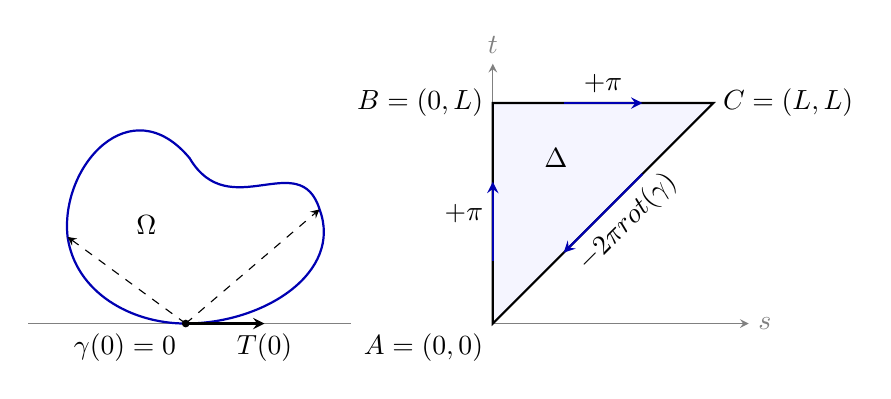
\begin{tikzpicture}[x=1cm,y=1cm,>=stealth]
	\begin{scope}[shift={(1.7,0.25)}]
		\draw[gray] (-2,0)--(2.1,0);
		\draw[thick,blue!70!black] (0,0) .. controls (1,0) and (2,0.65) .. (1.7,1.45) .. controls (1.45,2.25) and (0.55,1.25) .. (0.05,2.1) .. controls (-0.7,3) and (-1.6,2) .. (-1.5,1.1) .. controls (-1.4,0.4) and (-0.7,0) .. (0,0);
		\draw[->,thick] (0,0)--(1,0) node[below] {\(T(0)\)};
		\draw[dashed,->] (0,0)--(1.7,1.45);
		\draw[dashed,->] (0,0)--(-1.5,1.1);
		\fill (0,0) circle (1.4pt);
		\node[below left] at (0,0) {\(\gamma(0)=0\)};
		\node at (-0.5,1.25) {\(\Omega\)};
	\end{scope}
	\begin{scope}[shift={(5.6,0.25)}]
		\fill[blue!4] (0,0)--(0,2.8)--(2.8,2.8)--cycle;
		\draw[->,gray] (0,0)--(3.25,0) node[right] {\(s\)};
		\draw[->,gray] (0,0)--(0,3.3) node[above] {\(t\)};
		\draw[thick] (0,0)--(0,2.8)--(2.8,2.8)--cycle;
		\draw[->,blue!70!black,thick] (0,0.8)--(0,1.8);
		\draw[->,blue!70!black,thick] (0.9,2.8)--(1.9,2.8);
		\draw[->,blue!70!black,thick] (1.9,1.9)--(0.9,0.9);
		\node[left] at (0,1.4) {\(+\pi\)};
		\node[above] at (1.4,2.8) {\(+\pi\)};
		\node[rotate=45,below] at (1.5,1.5) {\(-2\pi\operatorname{rot}(\gamma)\)};
		\node at (0.8,2.1) {\(\Delta\)};
		\node[below left] at (0,0) {\(A=(0,0)\)};
		\node[left] at (0,2.8) {\(B=(0,L)\)};
		\node[right] at (2.8,2.8) {\(C=(L,L)\)};
	\end{scope}
\end{tikzpicture}

	\caption[弦方向的参数三角形]{左图以曲线最低点为基点，此点发出的所有弦均指向闭上半平面。右图的两条直角边分别记录基点弦方向及其负向，各有角增量 \(\pi\)；斜边逆向记录切向映射。图中曲线仅为示意，证明不要求凸性。}
	\label{g1:fig:chord-triangle}
\end{figure}

\begin{proof}
	先取弧长参数；\(C^1\) 正则性足以使用\cref{g1:prop:arc-length-param}，旋转次数不因这种保向重参数化而改变。旋转、平移平面并移动参数起点，使 \(\gamma(0)=\gamma(L)=0\) 是曲线第二坐标的最小点，整条曲线位于 \(y\geq0\)。该点的切向量水平。正向时 \(T(0)=(1,0)\)：最低点下方属于无界外部，局部内部在切线的上侧，正向要求它位于左方。

	在闭三角形
	\[
		\Delta=\{(s,t):0\leq s\leq t\leq L\}
	\]
	上定义一个圆周值映射。对 \(s<t\)、\((s,t)\ne(0,L)\)，令
	\[
		F(s,t)=\frac{\gamma(t)-\gamma(s)}{|\gamma(t)-\gamma(s)|}.
	\]
	简单性保证分母不为零。在对角线上令 \(F(s,s)=T(s)\)，在余下角点令 \(F(0,L)=-T(0)\)。这些赋值确实连续。对角线附近，
	\[
		\frac{\gamma(t)-\gamma(s)}{t-s}
		=\frac1{t-s}\int_s^t T(v)\,\mathrm{d}v
	\]
	一致趋近相应的单位切向量；这是紧区间上 \(T\) 一致连续的直接结果。在角点 \((0,L)\) 附近，设 \(a=s\)、\(b=L-t\)，由两端相容的导数 \(T(0)=T(L)\)，
	\[
		\gamma(L-b)-\gamma(a)=-(a+b)T(0)+o(a+b).
	\]
	归一化后恰趋向 \(-T(0)\)，也包括 \(a=0\) 或 \(b=0\) 的情形。

	令 \(A=(0,0)\)、\(B=(0,L)\)、\(C=(L,L)\)。沿 \(A\to B\) 走，\(F(0,t)\) 是从原点发出的弦方向，始终在闭上半圆。因此其连续角度可直接取为 \([0,\pi]\) 中的值，从 \(0\) 变到 \(\pi\)，总增量为 \(\pi\)。沿 \(B\to C\) 走，
	\[
		F(s,L)=-F(0,s),
	\]
	故在前一角度上加 \(\pi\)，得到从 \(\pi\) 到 \(2\pi\) 的提升，总增量仍为 \(\pi\)。沿 \(C\to A\) 的对角线走，方向映射为逆向的 \(T\)，总增量是 \(-2\pi\operatorname{rot}(\gamma)\)。

	另一方面，边界环路 \(F|_{\partial\Delta}\) 的总增量必须为零。具体地，把三角形边界上的点 \(x\) 沿 \((1-u)x+uA\) 缩到 \(A\)，再复合 \(F\)，就得到固定基点 \(F(A)\) 的零伦；\cref{g1:thm:circle-fundamental}说明它的绕数为零。三段角度相接，因而
	\[
		0=\pi+\pi-2\pi\operatorname{rot}(\gamma).
	\]
	这给出正向的结论。反向时旋转次数变号；\(C^2\) 情形的曲率积分再由\eqref{g1:eq:total-signed-curvature}得到。
\end{proof}

简单性在证明中有明确的用途：它保证任意两个不同参数点之间的弦方向都有定义。自交点会在三角形内部产生未定义点，边界映射就未必能延拓到整个三角形，绕数为零的论证也随之失效。

\subsection{曲率符号、凸性及反例}
\label{g1:subsec:0703:03}

若 \(k\geq0\)，切向角不减；再要求它只转一周，就能同时控制绕行次数并判断曲线的凸性。若一条简单闭曲线的像是某个有非空内部的紧凸集的边界，就称它为\term[tuquxian]{凸曲线}[convex curve]；这里允许边界包含线段。

\begin{theorem}[曲率符号与凸性]\label{g1:thm:curvature-convexity}
	设 \(L>0\)，\(\gamma:\mathbb R/L\mathbb Z\rightarrow\mathbb R^2\) 是 \(C^2\) 弧长参数正则闭曲线，平面取标准定向，以 \(k\) 记沿参数递增方向的有向曲率。
	\begin{enumerate}
		\item 若 \(k\geq0\) 且 \(\operatorname{rot}(\gamma)=1\)，则 \(\gamma\) 自动为简单闭曲线，且按正向恰好描出一个紧凸集的边界一周。
		\item 若已知 \(\gamma\) 是正向简单闭曲线，则它为凸曲线，当且仅当 \(k\geq0\)。
	\end{enumerate}
	相应地，反向时把 \(k\geq0\)、旋转次数 \(1\) 改为 \(k\leq0\)、旋转次数 \(-1\)。
\end{theorem}
\begin{proof}
	先假设 \(k\geq0\)、旋转次数为 \(1\)。切向角提升满足 \(\theta'=k\geq0\)、\(\theta(s+L)=\theta(s)+2\pi\)。任意选一个起点，平移和旋转后可设它的参数为 \(0\)、位置为 \(0\)、切向角为 \(0\)。记 \(\gamma(s)=(x(s),y(s))\)，则
	\[
		y'(s)=\sin\theta(s),\qquad 0\leq\theta(s)\leq2\pi,\qquad y(0)=y(L)=0.
	\]
	在切向角从 \(0\) 增至 \(\pi\) 的阶段，\(y\) 不减；从 \(\pi\) 增至 \(2\pi\) 的阶段，\(y\) 不增。因此 \(y(s)\geq0\)：整条曲线在所选起点的有向切线左侧。

	还须排除中途回到起点，不能仅由半平面包含关系断言简单性。若 \(0<\theta(s)\leq\pi\)，连续角度在此前经过 \((0,\pi)\) 中的一段，故 \(y(s)=\int_0^s\sin\theta(v)\,\mathrm{d}v>0\)。若 \(\pi\leq\theta(s)<2\pi\)，则
	\[
		y(s)=-\int_s^L\sin\theta(v)\,\mathrm{d}v>0.
	\]
	余下的 \(\theta(s)=0\) 情形，由单调性知 \([0,s]\) 上 \(T=(1,0)\)，所以 \(\gamma(s)=(s,0)\ne0\)；\(\theta(s)=2\pi\) 时，同理 \(\gamma(s)=(-(L-s),0)\ne0\)，这里均取 \(0<s<L\)。起点任意，所以两个不同参数类不可能具有同一像点，\(\gamma\) 为简单闭曲线。

	设其有界内部为 \(\Omega\)，\(K=\overline\Omega\)。转角定理表明当前参数为正向，故局部内部在左侧。前两段已经证明每一点的闭左半平面
	\[
		H_s=\{p:\langle p-\gamma(s),JT(s)\rangle\geq0\}
	\]
	包含整条曲线，也包含 \(K\)。后一断言可这样看：线性函数 \(\langle p-\gamma(s),JT(s)\rangle\) 在紧集 \(K\) 上取到最小值，若它为负且不在边界取到，就会在开集 \(\Omega\) 内有局部最小值，这与其非零线性梯度矛盾。

	事实上 \(K=\bigcap_sH_s\)。为证反向包含，取 \(p\notin K\)，在 \(K\) 中取距离 \(p\) 最近的点 \(q\)。最近点必在边界上，写 \(q=\gamma(s)\)；对 \(|p-\gamma(v)|^2\) 求导可知 \(p-q\perp T(s)\)。线段 \((q,p]\) 不碰 \(K\)，否则有更近的点。若 \(p-q\) 是左法向，线段靠近 \(q\) 的一小段就位于局部内部，与此矛盾。因此 \(p-q\) 是右法向，\(p\notin H_s\)。所求等式成立，而闭半平面的交是凸集。这证明第1项。

	现在假设曲线已简单并取正向。若 \(k\geq0\)，转角定理给出旋转次数 \(1\)，第1项适用。反之，设 \(K=\overline\Omega\) 凸。先说明每条切线都是支撑线。把任一边界点移到原点，使正向切向量为 \((1,0)\)，则附近边界写成 \(y=f(x)\)，其中 \(f(0)=f'(0)=0\)，局部 \(K\) 位于图像上方。如果某个 \(p=(p_x,p_y)\in K\) 满足 \(p_y<0\)，凸性使 \(tp\in K\) 对 \(0<t<1\) 成立。但 \(f(tp_x)=o(t)\)，故充分小时 \(tp_y<f(tp_x)\)，矛盾。因此 \(K\) 在切线的闭上半平面内，特别地 \(f(x)\geq0\)。于是 \(f''(0)\geq0\)。在这一坐标和方向下有向曲率为 \(f''(0)/(1+f'(0)^2)^{3/2}\)，所以 \(k\geq0\)。边界点任意，第2项得证。
\end{proof}

在证明中，允许 \(k=0\) 至关重要：它使 \(\theta\) 可以保持不变，对应曲线中的直线段。若正向简单闭曲线处处 \(k>0\)，则每条支撑切线只接触曲线一个点。事实上，对固定起点，切向角严格增加，证明中的法向高度在其余参数处都严格为正。因此此时所围凸集严格凸，即边界不包含非退化线段。逆命题却不成立：严格凸边界的个别点仍可以曲率为零，章末的四次曲线给出例子。

\begin{example}[正曲率仍可能重复绕行]\label{g1:exm:multiple-circle-turning}
	对整数 \(m\geq2\)，考虑 \(\gamma(t)=(\cos mt,\sin mt)\)，\(t\in\mathbb R/2\pi\mathbb Z\)。它正则，速率为 \(m\)，有向曲率恒为 \(1\)，但同一圆周被走了 \(m\) 遍。其总长为 \(2\pi m\)，旋转次数为 \(m\)。所以在尚未知道简单性时，不能把 \(k>0\) 直接当作简单凸曲线的判据。
\end{example}

\begin{example}[旋转一次仍可能有自交]\label{g1:exm:rotation-one-self-intersection}
	令
	\[
		\gamma(t)=(\cos t,\sin t+2\sin3t),\qquad t\in\mathbb R/2\pi\mathbb Z.
	\]
	当 \(\sin t\ne0\) 时，第一坐标导数 \(-\sin t\) 非零；在 \(t=0,\pi\) 处，第二坐标导数分别为 \(7,-7\)，故曲线处处正则。对 \(0<t<\pi\)，切向量的第一坐标为负，其角度可以连续取在 \((\pi/2,3\pi/2)\)，并从 \(\pi/2\) 走到 \(3\pi/2\)；对 \(\pi<t<2\pi\)，第一坐标为正，角度继续从 \(3\pi/2\) 走到 \(5\pi/2\)。两段合计增量 \(2\pi\)，所以旋转次数为 \(1\)。

	然而
	\[
		\sin t+2\sin3t=\sin t\,(8\cos^2t-1).
	\]
	选 \(t_0\in(0,\pi/2)\) 满足 \(\cos t_0=1/\sqrt8\)，就有 \(\gamma(t_0)=\gamma(2\pi-t_0)\)，因而曲线不简单。它的曲率也不是同号：\(\det(\dot\gamma,\ddot\gamma)\) 在 \(t=0\) 为 \(7\)，在 \(t=\pi/2\) 为 \(-17\)。这个例子把凸性判据的两个条件分开了：整周数为 \(1\) 只控制净转角，曲率符号才控制转向是否来回反复。
\end{example}

本节积分的是有向曲率，左转和右转会抵消。下一节改看 \(\int|k|\,\mathrm{d}s\) 及其空间曲线版本：即使净转角很小，实际弯曲的总量仍可能很大。
% 纲要条目排为编号小节标题，并进入目录与书签；说明段仍保留于纲要注释中。
